\documentclass[a4paper, oneside, 12pt]{article}

\usepackage{../custom}

\usepackage[backend=biber]{biblatex}
\addbibresource{biblio.bib}

\title{Tâche 2}
\author{Groupe 1225}
\date{\today}

\begin{document}

\maketitle

\section{Analyse des conditions optimales du réacteur de synthèse d'ammoniac}

Jusqu'ici nous avons considéré la dernière étape du procédé - la synthèse d'ammoniac -
comme une bo\^ite noire. Nous allons maintenant déterminer quelles sont les conditions 
optimales de température et de pression pour ce réacteur. 
Avant de commencer, il nous semble important de rappeler le principe 
de \textsc{Le Ch\^atelier} : \enquote{Si l'on tend à modifier les conditions d'un système en équilibre, 
il réagit de façon à s'opposer, en partie, aux changements qu'on lui impose, 
jusqu'à l'établissement d'un nouvel équilibre.}. \cite{chatelier}

La réaction de synthèse l'ammoniac est la suivante
\[\ce{N2_{(g)} + 3H2_{(g)} <=> 2NH3_{(g)} } \]

\paragraph{Pression}

On voit tout de suite que le nombre de moles de gaz de réactifs est supérieur 
au nombre de moles de gaz des produits, 
plus précisemment $n_{g}\text{(réactifs)} = 2 \cdot n_{g}\text{(produits)}$.

Par la loi des gaz parfait, on sais que la pression est directement proportionelle 
au nombre de moles de gaz. Le principe énoncé ci-dessus, 
nous permet de dire qu'une \emph{augmentation} de la pression du réacteur ($p_{\text{total}}$),
favorisera le sens de la diminution du nombre de moles de gazs, 
et dans notre cas, favorisera la production de \ce{NH3}.

\[
K = \frac{p_{eq,\ce{NH3}}^2}{p_{eq,\ce{H2}}^3 \cdot p_{eq,\ce{N2}} \cdot p_{\text{total}}^2}
\]
\paragraph{Température}

La réaction de synthèse est une réaction fortement exothermique 
(à $700\si{\kelvin}$, $\Delta_r H^{\circ} = -52.6\si{\kilo\joule}$).
Pour favoriser la réaction dans le sens de production des produits,
il faut donc faire une \emph{diminution} de la température.

\[
K = \exp{\left( \frac{- \Delta_r H^{\circ} + T \, \Delta_r S^{\circ}}{R T}\right)}
\]

\paragraph{Limite sur la température imposée par le catalyseur}

\paragraph{Limite sur la pression imposée par les matériaux du réacteur}

\section{Modélisation par Aspen +}
\subsection{Démarrage}

Lors de la première tâche, nous analysions l'installation dans son ensemble, 
mais de manière excessivement simplifiée. 
Dans cette section, nous nous concentrerons sur l'explicitation de la dernière étape 
pour ensuite la simuler sur le logiciel $Aspen Plus$. 
Nous ne désirons plus la considérer comme une boîte noire, et l'avons donc découpée 
en un certain nombre de processus intermédiaires. 

Le gaz composé d'\ce{N2}, d'\ce{H2} et d'\ce{Ar} passe par un réchauffeur et par un compresseur 
pour atteindre respectivement la température et la pression voulue. 
Il va ensuite dans le réacteur où se déroule la réaction.
Le produit est refroidit dans une installation prévue à cette fin, 
pour arriver enfin dans un séparateur où on extrait l'ammoniac.

Il semblait intéressant de créer un circuit de recyclage pour réutiliser 
le mélange de \ce{N_2} et de \ce{H_2} issus du processus (la réaction n'est pas complète 
et il reste donc des réactifs). Malheureusement, il y existe également de l'argon 
qu'on ne peut séparer du reste. En effet, sa température d'ébullition est bien trop 
proche de celle des autres composés et les moyens à mettre en œuvre en seraient 
très couteux et/ou à faible rendement.

Notre groupe a donc décidé de faire une purge dans le circuit de recyclage 
<<<<<<< HEAD
=======
afin d'éviter que l'argon ne s'accumule. Cette purge ne doit pas être trop 
grande sinon la quantité perdue des réactifs serait conséquente. 
La condition à respecter est donc d'avoir un flux entrant d'argon égal à celui de sortie:
Lors de la première tâche, nous analysions l'installation dans son ensemble, 
mais de manière excessivement simplifiée. Dans cette section, 
nous nous concentrerons sur l'explicitation de la dernière étape pour 
ensuite la simuler sur le logiciel \texttt{Aspen Plus}. 
Nous ne désirons plus la considérer comme une boîte noire, 
et l'avons donc découpée en un certain nombre de processus intermédiaires.

Le gaz composé d'$N_2$, d'$H_2$ et d'$Ar$ passe par un réchauffeur et 
par un compresseur pour atteindre respectivement la température et la pression voulue. 
Il va ensuite dans le réacteur où se déroule la réaction. 
Le produit est refroidit dans une installation prévue à cette fin, 
pour arriver enfin dans un séparateur où on extrait l'ammoniac. 

Il semblait intéressant de créer un circuit de recyclage pour réutiliser 
le mélange de $N_2$ et de $H_2$ issu du processus (la réaction n'est pas complète 
et il reste donc des réactifs). 
Malheureusement, il y existe également de l'argon qu'on ne peut séparer du reste. 
En effet, sa température d'ébullition est bien trop proche de celle des autres composés et 
les moyens à mettre en œuvre en seraient très couteux et/ou à faible rendement. 

Notre groupe a donc décidé de faire une purge dans le circuit de recyclage 
>>>>>>> origin/master
afin d'éviter que l'argon ne s'accumule. Cette purge ne doit pas être trop grande 
sinon la quantité perdue des réactifs serait conséquente. 
La condition à respecter est donc d'avoir un flux entrant d'argon égal à celui de sortie. 
Les calculs permettant de trouver la quantité parfaite à purger 
sont détaillés dans la sous-section suivante.

Voici à quoi ressemble l'installation sur $ASPEN$:
[INSERER PRINTSCREEN]

\subsection{La purge}

Dans les calculs qui suivent, nous cherchons $x$ qui n'est autre que la fraction du recyclage 
qui doit être purgée. Nous nous référerons au schéma pour ce qu'il en est des notations. 
Rappelons qu'il est aisé de trouver les débits d'entrée des réactifs 
et de sortie de l'ammoniac grâce à notre outil de calcul.

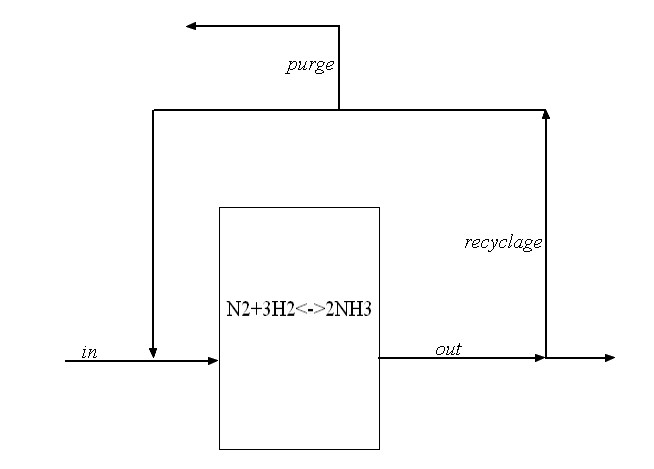
\includegraphics[scale=0.5]{etape_finale_simpl.jpg} 

Comme dit précédemment, une purge optimale doit permettre un débit 
de sortie d'argon égal à celui d'entrée dans le système. 
On peut écrire ça sous la forme:

\begin{equation}
\dot{n}_{Ar,in}=\dot{n}_{Ar,purge}=[Ar]_{purge} \dot{n}_{purge}
\end{equation}

Ceci est donc le bilan total d'argon. 
Il est possible de faire d'autres bilans afin de nous donner d'autres relations utiles.

$\bullet$ Bilan molaire à la purge:
\begin{equation}
\dot{n}_{purge} = x \cdot \dot{n}_{recyclage}
\label{eq:bilan_mol_purge}
\end{equation}

$\bullet$ Bilan molaire au séparateur:
\begin{equation}
\dot{n}_{out}=\dot{n}_{recyclage}+\dot{n}_{NH_3,out}
\end{equation}

$\bullet$ Bilan d'argon au séparateur:
\begin{equation}
[Ar]_{out} \dot{n}_{out}=[Ar]_{recyclage} \dot{n}_{recyclage}
\end{equation}

$\bullet$ Bilan molaire total:

\begin{equation}
	\dot{n}_{in} - 2\xi=\dot{n}_{NH_3,out} + \dot{n}_{purge}
\end{equation}

avec $\xi$ étant l'avancement, c'est à dire le nombre de moles de $N_2$ ayant réagit. 
Faisons attention de noter qu'on ne considère que les réactifs venant du circuit $in$. 
Cela est résumé dans le tableau suivant. 
On analyse le débit de moles à l'entrée du réacteur pour les différents composés, 
ainsi qu'à la sortie (on considère que l'équilibre a été atteint).

\begin{table}
	\centering
	\begin{tabular}{l|c|c|c|c}
		$\ce{N2}$ & $\ce{H2}$ & $\ce{Ar}$ & $\ce{NH3}$ & $n_{total}$ \\
		\hline
		$n_{\ce{N2},in}$ & $n_{\ce{H2},in}$ & $n_{\ce{Ar},in}$ & $0$  & $n_{in}$\\
		$n_{\ce{N2},in}-\xi$ & $n_{\ce{H2},in}-3\xi$ & $n_{\ce{Ar},in}$ & $2\xi$  & $n_{in}-2\xi$\\
	\end{tabular}
	\caption{Réaction dans le réacteur}
	\label{tab:reaction1_primaire}
\end{table}

La réaction se déroule à $750K$ et 
il est facile de calculer $K en trouvant $\Delta G_{réaction}$ au préalable. 
Nous pouvons faire cela en utilisant notre outil de calcul.

\[
K=\exp(\frac{-\Delta G}{R\cdot 750})\]

L'expression de la constante d'équilibre $K_p$ est également: 

\[
K_p=\frac{{[NH_3]_{out}}^2}{[N_2]_{out}{[H_2]_{out}}^3} = 
\frac{{n_{NH_3,out}}^2}{n_{N_2,out}\cdot {n_{H_2,out}}^3}\cdot {n_{total,out}}^2\cdot p_{réacteur}
\]

Comme $n_{H_2}=3\cdot n_{N_2}$ (éléments en quantité stœchiométrique), on a donc 
$K==\frac{{n_{NH_3,out}}^2}{27{n_{N_2,out}}^4}\cdot {n_{total,out}}^2$. En injectant les 
quantités de composés du tableaux, fonctions de $\xi$, on obtient:

\[ K=\frac{{2\xi}^2}{27{{n_{N2}-\xi}^4}}\cdot {n_{total}-2\xi}^2 \]
Nous pouvons par exemple résoudre cela avec $MATLAB$. 
Connaissant $\xi$, on trouve $\dot{n}_{purge}$ grâce à l'équation(5). 
Nous obtenons directement $[Ar]_{purge}$ en injectant 
le résultat dans la première équation. $[Ar]_{purge}$ est égal à $[Ar]_{recyclage}$ 
car la purge n'altère par la concentration.

Nous disposons de la quantité d'ammoniac produite (un paramètre) 
et pouvons donc maintenant connaitre la quantité totale de réactifs restants après réaction. 
Rappelons que les quantité utilisées plus haut ne prenaient pas en compte le recyclage. 
Reprenons l'expression de K: 

\[ K==\frac{{n_{NH_3,out}}^2}{27{n_{N_2,out}}^4}\cdot {n_{total,out}}^2\cdot p_{réacteur} \]

$n_{total,out}=4n_{N_2,out}+n_{Ar,out}$ 
avec $n_{Ar,out}=n{Ar,in}+n{Ar,recyclage}=n{Ar,in}+[Ar]_{recyclage}n{total,recyclage}\underset{(3)}=n{Ar,in}+[Ar]_{recyclage}(n{total,out}-n_{NH_3,out}$.

Nous avons donc 2 équation pour trouver les 2 inconnues $n_{N_2,out}$ et $n_{total,out}$. 
Nous pouvons à nouveau résoudre cela par $MATLAB$. 
A présent, il suffit d'utiliser l'équation (3) pour trouver $\dot{n}_{recyclage}$. 
Comme nous le dit l'équation \ref{eq:bilan_mol_purge}, le rapport de $\dot{n}_{purge}$ 
et de $\dot{n}_{recyclage}$ nous donne enfin x! 
Ces calculs fastidieux nous permettent donc enfin de trouver la fraction à prélever 
dans le circuit de recyclage. 
Le même cheminement est suivi dans le programme \texttt{purge} disponible dans notre outil de gestion.

\subsection{Validation du modèle}

Le logiciel $ASPEN$ propose de nombreuses modélisations du comportement des fluides, 
plus ou moins fidèles selon les composés et les conditions dans lesquels on les observe. 
Notre recherche s'est limitée aux modèle à haute pression. 
Après en avoir fait l'étude en comparant les bases de données de chacun d'eux, 
nous nous sommes arrêtes sur le modèle REFPROP, acronyme pour REFerence fluid PROPerties. 
Ce dernier est actuellement le modèle le plus précis existant. 
Il implémente les équations d'état de Helmholtz, de Benedict-Webb-Rubin 
et d'un modèle étendu de correspondance d'états (ECS) tout en s'appuyant sur des résultats expérimentaux. 
Il fonctionne pour les composés purs comme pour pour les mélanges, 
et ce en particulier pour une grande liste de réactifs qui comprend tout ceux intervenant dans notre cas. 
Pour toutes ces raisons, le choix de ce modèle a paru judicieux.

Pour lancer une simulation de notre installation, 
nous avons fixé nos paramètres à des valeurs vraisemblables 
et observé le comportement suivi dans le programme. 
[AJOUTER LES RESULTATS DONNES PAR LA SIMULATION]

\printbibliography
\end{document}

